\documentclass[11pt]{amsart}
\usepackage[margin=1.1in]{geometry}
\usepackage{amsmath,amssymb,amsthm,booktabs,enumitem,graphicx}
\usepackage[colorlinks=true,linkcolor=blue,citecolor=blue,urlcolor=blue]{hyperref}
\graphicspath{{../figures/}}
\allowdisplaybreaks
\setlength{\emergencystretch}{2.5em}
\newtheorem{theorem}{Theorem}[section]
\newtheorem{proposition}[theorem]{Proposition}
\newtheorem{lemma}[theorem]{Lemma}
\newtheorem{corollary}[theorem]{Corollary}
\newtheorem{hypothesis}[theorem]{Hypothesis}
\theoremstyle{remark}
\newtheorem{remark}[theorem]{Remark}
\newcommand{\Z}{\mathbb Z}
\newcommand{\Q}{\mathbb Q}
\newcommand{\e}{\varepsilon}
\newcommand{\cA}{\mathcal A}
\newcommand{\cE}{\mathcal E}
\newcommand{\cP}{\mathcal P}
\newcommand{\cM}{\mathcal M}
\DeclareMathOperator{\Cl}{Cl}

\title[Sums of two squares and Heegner norms, XIV]{Sums of two squares and Heegner norms with few prime factors, XIV:\\ the Buchstab fixed point of a vector sieve as an obstacle problem,\\ causal computation, and variable dispersion levels}
\author{Ruqing Chen}
\address{GUT Geoservice Inc., Montreal, Canada}
\email{ruqing@hotmail.com}
\date{\today\ (draft)}

\begin{document}
\begin{abstract}
Part~XIII sifted $N-p$ by two semi-linear sieves (split primes below $N^\eta$, inert primes below $N^\theta$) in a vector sieve, iterated Buchstab's identity on the inert primes, and obtained $N=Q_{C'}(u,v)_{\rm prime}+Q_C(x,y)_{P_r}$ with $r_0(L)=7,10,16$ for the switching losses $L=1,\frac32,3$. Here we study the fixed point of that recursion. In the gauge $u=a^{-1/2}\Phi$, $v=a^{-1/2}G$ it is an obstacle problem of Hamilton--Jacobi--Bellman type on the half-plane of levels $X$ and inert exponents $a$: either the rectangle bound is active or the pure delay equation $-a\,\partial_au=\frac12a^{-1/2}G(X-a;e,a)$ holds. The equation is causal in the level, so the fixed point is computed in one sweep in $O(n^2)$ operations instead of $O(mn^3)$; it agrees with the iteration of Part~XIII to machine precision and runs $2000$ times faster. We prove a half-level scaling law, $G(X;e,a)=\sqrt{2a/X}\,G(X;e,X/2)$ for $a\ge X/2$, which reduces the storage to $O(n^2/6)$ entries, and we observe that the free boundary degenerates: the optimal cut is the smallest admissible one on the whole active region $a<X-1.5e$. With grids up to $n=12800$ and a one-sided quadrature that errs on the safe side, the thresholds at the Bombieri--Vinogradov level $\frac12$ become $r_0(L)=7,9,15$, so the $D=23$ table of Part~XIII becomes $9/8$, $11/10$, $17/16$. Under a level of distribution of Lichtman's type for the switched sequence $\{q_1q_2r\}$, uniform in the residue $N$ (Hypothesis~L, which we reduce to Lichtman's bilinear and divisor estimates), the thresholds are $6,8,14$: every large even admissible $N$ is $p+x^2+y^2$ with $\Omega(x^2+y^2)\le6$. Finally the same engine with a linear auxiliary sieve treats the problem $p-1=m^2+n^2$, $p+2=P_r$ of Nath and Xie. Their numerical value rests on an incorrect delay system for the linear sieve functions; with the correct functions their inequality gives $r=84$, and the fixed point gives $r=65$ (one-sided) and $56$ (trapezoid).
\end{abstract}
\maketitle

\section{Introduction}
Part~XIII \cite{ChenXIII} proved statements of the shape
\begin{equation}\label{eq:shape}
N=Q_{C'}(u,v)+Q_C(x,y),\qquad Q_{C'}(u,v)=p\ \text{prime},\qquad\Omega(Q_C(x,y))\le r,
\end{equation}
for every large admissible $N$, with explicit $r$. The sieve is a vector sieve of two semi-linear sieves on $m=N-p$: the split primes below $z_1=N^\eta$ and the inert primes below $z_3=N^\theta$, $\frac14<\theta<\frac12$, at the Bombieri--Vinogradov level $N^{1/2-\e}$ (Theorem~1.1 of Part~XIII for the primes of one form). The bad survivors $m=q_1q_2r$ with two large inert primes are removed by Chen's switching, which costs the factor $L=L_{C'}\in\{1,\frac32,3\}$, and the number of prime factors is controlled by Richert's weights. Lemma~4.3 of Part~XIII iterated Buchstab's identity on the inert primes: with
\begin{gather*}
\Phi_0(X;e,a)=\max_{\substack{es_1+as_3=X\\ s_1,s_3\ge1}}\bigl[f(s_1)F(s_3)+F(s_1)f(s_3)-F(s_1)F(s_3)\bigr]^+,\\
G_0(X;e,a)=\min_{es_1+as_3=X}F(s_1)F(s_3),
\end{gather*}
the recursion
\begin{align}
\Phi_m(X;e,a)&=\max_{0<\theta_0\le a}\Bigl[\sqrt{\tfrac a{\theta_0}}\,\Phi_0(X;e,\theta_0)-\frac12\int_{\theta_0}^{a}\sqrt{\tfrac ab}\,G_{m-1}(X-b;e,b)\,\frac{db}b\Bigr]\quad(X>a),\label{eq:recP}\\
G_m(X;e,a)&=\min_{0<\theta_0\le a}\Bigl[\sqrt{\tfrac a{\theta_0}}\,G_0(X;e,\theta_0)-\frac12\int_{\theta_0}^{a}\sqrt{\tfrac ab}\,\Phi_{m-1}(X-b;e,b)\,\frac{db}b\Bigr]\label{eq:recG}
\end{align}
gives valid lower and upper bounds for every $m$, monotone in $m$, and the criterion of Proposition~4.2 there,
\begin{equation}\label{eq:crit}
\cM=\frac{e^{-\gamma}}{\sqrt{\eta\theta}}\Bigl[\Phi(\tfrac12;\eta,\theta)-\frac\lambda2\int_\eta^{u_0}\Bigl(1-\frac t{u_0}\Bigr)G(\tfrac12-t;\eta,\theta)\frac{dt}t\Bigr]-8LJ_\lambda(\eta,\theta)>0
\end{equation}
with $\frac1\lambda+\frac1{u_0}\le r+1$, gave $r_0(L)=7,10,16$ at the fixed point ($m=12$, grid $n=1600$).

This paper is about the fixed point itself. Three things are new.

\emph{The structure.} In the gauge $u=a^{-1/2}\Phi$, $v=a^{-1/2}G$ the fixed point is an obstacle problem (Section~\ref{sec:obstacle}): at every $(X,a)$ either the rectangle bound is active or the delay equation $-a\,\partial_au=\frac12a^{-1/2}G(X-a;e,a)$ holds, and likewise for $v$ with $\Phi$. The equation is \emph{causal in the level}: the row $X$ only reads rows below $X$. So the fixed point, which the iteration of Part~XIII reaches only after $m=n$ steps on a grid of $n$ levels, is computed in one upward sweep, and inside a row the search for the cut is a cumulative maximum. The cost drops from $O(mn^3)$ to $O(n^2)$ (Proposition~\ref{prop:causal}), the result agrees with the iteration to $10^{-14}$, and $n=1600$ takes $0.3$ seconds instead of $576$. A half-level scaling law (Proposition~\ref{prop:half}) removes three quarters of the storage. Numerically the free boundary degenerates: on the whole active region $a<X-1.5e$ the optimal cut is the smallest admissible one, so the fixed point is the solution of the pure delay system with the rectangle bound only as a boundary condition (Section~\ref{sec:phase}).

\emph{Level $\frac12$.} With grids up to $n=12800$ and a one-sided cell rule that errs on the safe side (Section~\ref{sec:half}), the thresholds of Part~XIII improve by one for $L=\frac32$ and $L=3$.

\begin{theorem}\label{thm:half}
At the level of distribution $N^{1/2-\e}$ the criterion \eqref{eq:crit} holds, with the fixed point of \eqref{eq:recP}--\eqref{eq:recG} and a margin certified by the one-sided rule, for
\[
r_0(1)=7,\qquad r_0(\tfrac32)=9,\qquad r_0(3)=15 .
\]
Consequently, in Theorem~1.4 of Part~XIII ($D=23$) the table becomes $9/8$, $11/10$, $17/16$ for the rows $p$ arbitrary, $C'$ non-principal, $C'$ principal, and Theorems~1.2, 1.3 and Corollary~1.5 of Part~XIII hold with these values of $r_0$.
\end{theorem}
The margins of $r=9$ and $r=15$ are $0.5\%$ and $0.7\%$ of the main term, against $10\%$ for $r=7$; the next values $r=6$, $8$, $14$ fail by $9\%$, $12\%$ and $6\%$.

\emph{Variable level.} The switched term is the count of $n=q_1q_2r$ (inert $q_1<q_2$, $r$ a product of split primes) with $N-q_0^an$ prime, bounded by the linear upper sieve at level $N^{1/2}$ with the constant $F_{\rm lin}(1)=2e^\gamma$. Levels beyond $\frac12$ for well-factorable weights (Fouvry--Iwaniec, Bombieri--Friedlander--Iwaniec \cite{FI,BFI}) require a fixed residue class; the residue here is $N\overline{q_0^a}$, of size $N$. Lichtman \cite{Lichtman} removed this restriction for the primes, with a level $\vartheta_1(t)$ that depends on the largest prime factor $N^{t}$ of the modulus and peaks at $153/256$, uniformly for residues $|a|<x^{1+\e}$; Runbo Li \cite{Li} used it for Chen-switched sets of products of primes and raised Chen's Goldbach constant from $0.899$ to $1.97$. Section~\ref{sec:level} states the corresponding level for our $\cE=\{q_1q_2r\}$ as Hypothesis~\ref{hyp:L} and reduces it to Lichtman's two estimates (Propositions~3.1 and~3.2 of \cite{Lichtman}) by a double Heath-Brown decomposition.

\begin{theorem}\label{thm:level}
Assume Hypothesis~\ref{hyp:L}. Then the switched term carries the factor $G_1/(4e^\gamma)$ of Section~\ref{sec:level} in place of $1$, and the criterion holds for
\[
r_0(1)=6,\qquad r_0(\tfrac32)=8,\qquad r_0(3)=14 ,
\]
both with Li's value $G_1=6.069$ and with our recomputed value $G_1=5.581$. In particular every large even admissible $N$ is $p+x^2+y^2$ with $\Omega(x^2+y^2)\le6$ for $D=4$, and $N=Q(u,v)_{\rm prime}+Q(x,y)_{P_6}$ for the nine fields of class number one; the $D=23$ table becomes $8/7$, $10/9$, $16/15$.
\end{theorem}

\emph{Another dimension.} The engine of Section~\ref{sec:obstacle} takes an auxiliary sieve of dimension $\frac12$ or $1$. With dimension $1$ it treats the problem of Nath and Xie \cite{NX}: primes $p$ with $p-1=m^2+n^2$ and $p+2=P_r$, where the inert primes $q\equiv3\pmod 4$ are sifted from $p-1$ and all primes below $N^{\theta_2}$ from $p+2$. Their Theorem~1.1 states $r=9$. Section~\ref{sec:nx} shows that the numerical value behind it, $H(0.17,0.25,0.449,0.011)=1.2690$, comes from an incorrect delay system for the linear sieve functions in their computation files (the factor $1/s$ is missing, so that their lower function exceeds their upper function at $s=3$), and that with the correct functions $H=-24.9$ at that point. With the correct functions their inequality gives $r=84$; our fixed point gives the following.

\begin{theorem}\label{thm:nx}
With the sieve of \cite{NX} at the level $x^{1/2}$ and the fixed point of \eqref{eq:recP}--\eqref{eq:recG} on the inert primes of $p-1$ (auxiliary linear sieve on $p+2$), there are $\gg x(\log x)^{-5/2}$ primes $p\le x$ with $p-1$ a sum of two squares and $\omega(p+2)\le65$, $p+2$ squarefree. The trapezoid rule gives $56$ at the same grid.
\end{theorem}
The bottleneck there is the switched term of \cite{NX}, which is bounded by a product of two linear upper sieves; the vector sieve is not the limiting factor.

\subsection*{Conventions}
$f,F$ are the functions of the half-dimensional sieve (Part~XIII, Section~4.3) and $f_1,F_1$ those of the linear sieve, $F_1(s)=2e^\gamma/s$ on $(0,3]$, $f_1(s)=2e^\gamma\log(s-1)/s$ on $[2,4]$, continued by $(sF_1)'=f_1(s-1)$ and $(sf_1)'=F_1(s-1)$. The auxiliary sieve has dimension $\kappa_{\rm aux}\in\{\frac12,1\}$, exponent $e$, functions $f_{\rm aux},F_{\rm aux}$; the main sieve has dimension $\frac12$ and exponent $a$. $X$ is the level exponent. The grid is $X=ih$, $a=jh$, $h=1/(2n)$, $1\le i\le n$, $1\le j<n$.

\section{The fixed point as an obstacle problem}\label{sec:obstacle}
\subsection{Gauge and variational inequalities}
Put $u(X,a)=a^{-1/2}\Phi(X;e,a)$, $v(X,a)=a^{-1/2}G(X;e,a)$ and the obstacles $\psi^-=a^{-1/2}\Phi_0$, $\psi^+=a^{-1/2}G_0$. Dividing \eqref{eq:recP}--\eqref{eq:recG} by $\sqrt a$ removes every $a$ from the kernel:
\begin{align}
u(X,a)&=\max_{0<\theta_0\le a}\Bigl[\psi^-(X,\theta_0)-\frac12\int_{\theta_0}^ab^{-3/2}G(X-b;e,b)\,db\Bigr],\label{eq:u}\\
v(X,a)&=\min_{0<\theta_0\le a}\Bigl[\psi^+(X,\theta_0)-\frac12\int_{\theta_0}^ab^{-3/2}\Phi(X-b;e,b)\,db\Bigr].\label{eq:v}
\end{align}
At a fixed level $X$ these are Bellman equations in the single variable $a$: moving from $a'$ to $a>a'$ with the same cut subtracts $\frac12\int_{a'}^ab^{-3/2}G(X-b;e,b)db$, and at $a$ one may instead stop at the obstacle. So the fixed point satisfies, wherever $u$ is differentiable in $a$,
\begin{gather}
\min\Bigl\{u-\psi^-,\ -a\,\partial_au-\tfrac12a^{-1/2}G(X-a;e,a)\Bigr\}=0,\label{eq:hjb}\\
\min\Bigl\{\psi^+-v,\ -a\,\partial_av-\tfrac12a^{-1/2}\Phi(X-a;e,a)\Bigr\}=0 ,\notag
\end{gather}
the first factor vanishing on the stopping set (the cut is $\theta_0=a$) and the second on the continuation set, with the free boundary between them. The two problems are coupled only through the delayed terms $G(X-a;e,a)$ and $\Phi(X-a;e,a)$, which live at the lower level $X-a$.

\subsection{Causality}
\begin{proposition}[causality]\label{prop:causal}
On the grid, let $\Phi^{(i)},G^{(i)}$ denote the rows at level $X=ih$ of the fixed point. Then $\Phi^{(i)}$ and $G^{(i)}$ are determined by the rows $\Phi^{(i')},G^{(i')}$ with $i'<i$ through \eqref{eq:u}--\eqref{eq:v}, and the iteration $(\Phi_m,G_m)$ of Part~XIII reaches its fixed point in row $i$ exactly at $m=i$. Within a row, with $c_k=\psi^-(i,k)$ and $K_j=\sum_{l<j}(a_l^{-1/2}-a_{l+1}^{-1/2})\,{\rm cell}(i,l)$,
\[
u(i,j)=\max_{k\le j}\bigl[c_k-(K_j-K_k)\bigr]=\max_{k\le j}(c_k+K_k)-K_j ,
\]
a cumulative maximum, and likewise $v$ with a cumulative minimum. Hence one upward sweep over $i$ computes the fixed point in $O(n^2)$ operations.
\end{proposition}
\begin{proof}
The integrands in \eqref{eq:u}--\eqref{eq:v} are $G(X-b;e,b)$ and $\Phi(X-b;e,b)$ with $b\ge h$, i.e.\ rows $X-b<X$. If rows $i'<i$ are at their fixed point when row $i$ is computed, row $i$ is at its fixed point; by induction on $i$ the sweep gives the fixed point, and in the iteration of Part~XIII row $1$ is fixed from $m=1$ on (it only reads $\Phi_0,G_0$) and row $i$ from $m=i$ on. The cumulative form follows from $K_j-K_k=\sum_{k\le l<j}$.
\end{proof}
Here ${\rm cell}(i,l)$ is the value assigned to the cell $[a_l,a_{l+1}]$ of the $b$-integral: the mean of the two endpoint values $G(X_i-a_l;e,a_l)$, $G(X_i-a_{l+1};e,a_{l+1})$ (trapezoid rule, exact measure $\frac12\int\sqrt{a/b}\,db/b$ on the cell), or the larger endpoint value in the term subtracted from $\Phi$ and the smaller one in the term subtracted from $G$ (one-sided rule). The one-sided rule is rigorous whenever the integrand is monotone on the cell, and it converges from the safe side like $h$ (Section~\ref{sec:half}).

The sweep was checked against the iteration of Part~XIII (\texttt{code/hjb\_sieve\_engine.py verify}): on the same rectangle tables the two agree to $1.9\cdot10^{-7}$ at $m=12$ (the iteration is not yet converged there) and to $7\cdot10^{-15}$ at $m\ge30$. On $n=1600$ the sweep takes $0.27$ seconds against $576$ seconds for twelve steps of the iteration; the rectangle tables themselves, which are maxima and minima over $s_1$-grids and hence valid bounds on every grid, take $27$ seconds with $120$ points.

\subsection{Half-level scaling}
\begin{proposition}[half-level scaling]\label{prop:half}
For $a\ge X/2$, $\Phi(X;e,a)=0$ and
\[
G(X;e,a)=\sqrt{\frac{2a}{X}}\;G\Bigl(X;e,\frac X2\Bigr).
\]
The same holds for $G_0$, and on the grid for the computed fixed point.
\end{proposition}
\begin{proof}
$\Phi_0(X;e,a)=0$ for $X\le a+e$, so $\Phi(X;e,a)=0$ for $a\ge X/2$ once $X\le 2e$ is excluded by the definition; in any case $\Phi(X-b;e,b)=0$ for $b\ge X/2$, since $X-b\le b$. For $a\ge X/2$ every $s_3=(X-es_1)/a$ is at most $2$, where $F(s_3)=2e^{\gamma/2}(\pi s_3)^{-1/2}\propto\sqrt a$ with the same minimising $s_1$ for all such $a$; so $\psi^+(X,a)=a^{-1/2}G_0(X;e,a)$ is constant on $a\ge X/2$. In \eqref{eq:v} the integrand vanishes for $b\ge X/2$ and $\psi^+(X,\theta_0)$ is constant for $\theta_0\ge X/2$, so $v(X,a)=v(X,X/2)$ for $a\ge X/2$. On the grid the same argument applies cell by cell.
\end{proof}
Consequently the row $i$ of $G$ needs to be computed only for $j\le\lceil i/2\rceil$ and stored as the scalar $v(i,\lceil i/2\rceil)$ beyond. Together with the storage by anti-diagonals $i+j\le n$ (row $i'$ reads exactly the anti-diagonal $i+l=i'$) the tables occupy $n^2/6+n^2/4$ entries: $4$~MB at $n=1600$ and $256$~MB at $n=12800$ in single precision, with the row computations in double precision (\texttt{code/causal\_fixed\_point.py lowmem}).

\subsection{The free boundary}\label{sec:phase}
The optimal cuts $\theta_0^*(X,a)$ of the fixed point were recorded on $n=1600$ for $e=0.011$ and $e=0.005$ (Figure~\ref{fig:phase}). The picture is simple.
\begin{itemize}[leftmargin=1.5em]
\item The stopping set of $u$ (the rectangle bound is active, $\theta_0^*=a$) is the strip $X-c(e)e\le a<X$ with $c(0.011)=1.48$ and $c(0.005)=1.50$, independent of $X$. At the top level $X=\frac12$ the strip starts at $a=0.4838$ for $e=0.011$ and at $a=0.4925$ for $e=0.005$.
\item On the active region $a<X-c(e)e$ the optimal cut is the smallest admissible one, $\theta_0^*=h$, for $\Phi$ and for $G$ alike, at every level $X\ge0.1$; so there the fixed point solves the pure delay equations in \eqref{eq:hjb} with the obstacle entering only through the boundary value at $\theta_0=h$.
\item Interior cuts $\theta_0^*>h$ occur only at low levels, $X/e\lesssim6$ ($X\le0.07$ for $e=0.011$, none for $e=0.005$ down to $X=0.03$). There the bracket with cut $\theta_0$ behaves like $\theta_0^{-1/2}$ times $f_{\rm aux}(X/e)-F_{\rm aux}(X/e)$ as $\theta_0\to0$, and this difference is no longer negligible at $s=X/e$.
\end{itemize}
Two consequences. First, as $h\to0$ the cut moves to $0$, so the dependence on $n$ in Section~\ref{sec:half} is a genuine effect of the admissible cuts, not only a quadrature error; the margins increase monotonically with $n$ and converge like $h$ for both rules. Second, Lemma~4.3 of Part~XIII is best read as follows: the inert primes are handled entirely by Buchstab's identity, down to the smallest scale, and the vector sieve only serves the split primes.

\begin{figure}[htbp]
\centering
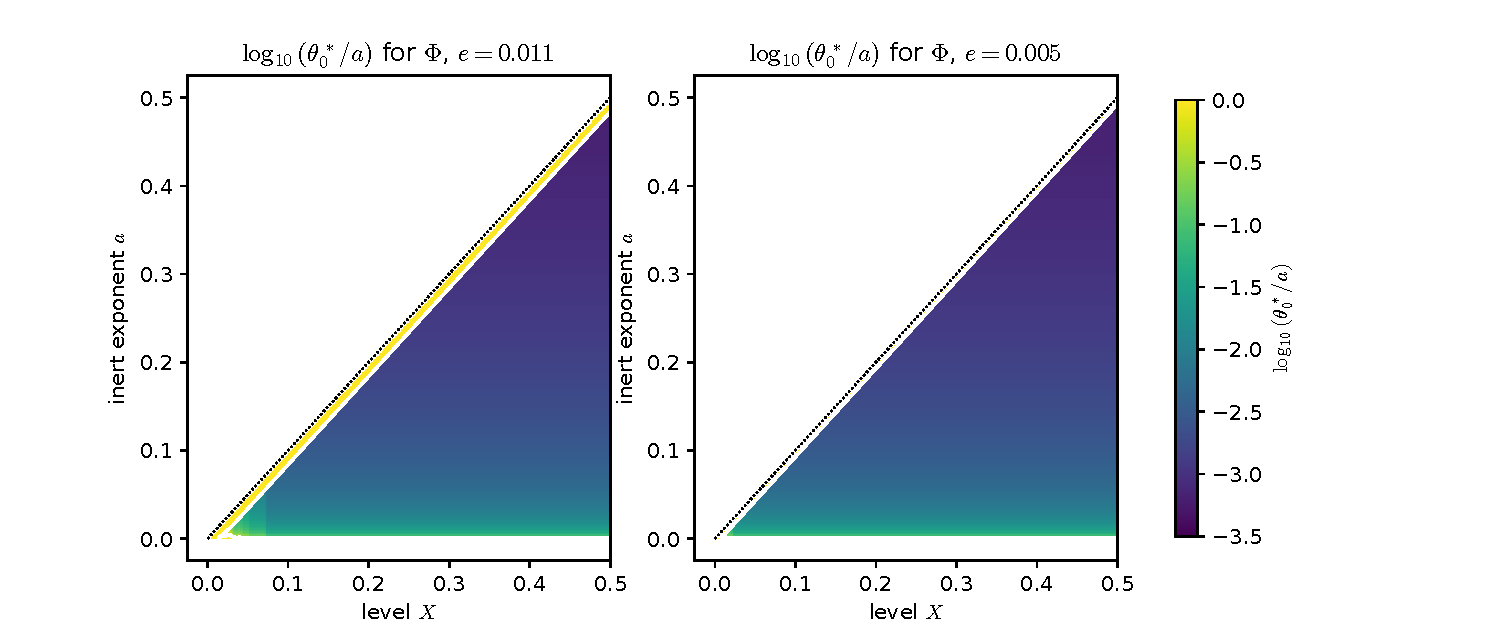
\includegraphics[width=\textwidth]{hjb_phase.pdf}
\caption{$\log_{10}(\theta_0^*/a)$ for $\Phi$ at the fixed point, $n=1600$, trapezoid rule, for $e=0.011$ (left) and $e=0.005$ (right). White: the stopping strip $a\ge X-1.5e$, where the rectangle bound is active. On the coloured region the cut is the smallest admissible one, $\theta_0^*=h=1/3200$.}
\label{fig:phase}
\end{figure}

\section{Level one half}\label{sec:half}
Table~\ref{tab:half} gives the margin $\cM$ of \eqref{eq:crit} at the fixed point on $n=1600$, $3200$, $6400$ and, for $r=15$, $12800$, with both cell rules, at the parameters of the retuning of Part~XIV's preparatory runs ($\eta$ in steps of $0.001$, $\theta$ in steps of $0.0025$, $u_0$ optimised). The one-sided values increase like $h$ (the ratios of successive differences are $0.99$--$1.01$) and the trapezoid values converge from below as well; Richardson extrapolation of the two rules agrees to $5\cdot10^{-4}$.

\begin{table}[htbp]
\centering\footnotesize\setlength{\tabcolsep}{3.5pt}
\begin{tabular}{ccccc|cccc|cccc|c}
\toprule
& & & & & \multicolumn{4}{c|}{trapezoid rule} & \multicolumn{4}{c|}{one-sided rule} & \\
$L$ & $r$ & $\eta$ & $\theta$ & $u_0$ & $1600$ & $3200$ & $6400$ & $12800$ & $1600$ & $3200$ & $6400$ & $12800$ & limit\\
\midrule
$1$ & $7$ & $0.015$ & $0.370$ & $0.329$ & $+0.273$ & $+0.274$ & $+0.274$ & & $+0.237$ & $+0.256$ & $+0.265$ & & $+0.274$\\
$1$ & $6$ & $0.015$ & $0.370$ & $0.377$ & $-0.186$ & $-0.186$ & $-0.185$ & & $-0.224$ & $-0.204$ & $-0.195$ & & $-0.185$\\
$\frac32$ & $10$ & $0.010$ & $0.420$ & $0.268$ & $+0.299$ & $+0.301$ & $+0.301$ & & $+0.241$ & $+0.272$ & $+0.287$ & & $+0.301$\\
$\frac32$ & $9$ & $0.011$ & $0.4175$ & $0.290$ & $+0.024$ & $+0.025$ & $+0.026$ & & $-0.031$ & $-0.003$ & $+0.012$ & & $+0.026$\\
$3$ & $16$ & $0.005$ & $0.460$ & $0.199$ & $+0.182$ & $+0.186$ & $+0.188$ & & $+0.061$ & $+0.125$ & $+0.157$ & & $+0.189$\\
$3$ & $15$ & $0.005$ & $0.4625$ & $0.219$ & $+0.024$ & $+0.027$ & $+0.029$ & $+0.030$ & $-0.102$ & $-0.036$ & $-0.003$ & $+0.014$ & $+0.030$\\
\bottomrule
\end{tabular}
\caption{The margin $\cM$ at the fixed point, level $\frac12$, in units of $2\mathcal B$. The limit is the Richardson extrapolation (order $1$) of the one-sided values. The certified values are the one-sided ones on the finest grid: $r=9$ is positive from $n=6400$ on and $r=15$ from $n=12800$ on.}
\label{tab:half}
\end{table}

\begin{proof}[Proof of Theorem~\ref{thm:half}]
The one-sided values on the finest grids are positive for $r=7,9,15$: $+0.265$ ($n=6400$), $+0.012$ ($n=6400$) and $+0.014$ ($n=12800$, where the trapezoid rule gives $+0.030$ and the tables occupy $273$~MB). By Lemma~4.3 of Part~XIII with the fixed point in place of $\Phi_m,G_m$ (the fixed point is a limit of valid bounds, Section~4.7 there), Proposition~4.2 of Part~XIII applies with these $r$. The $D=23$ table follows as in Part~XIII with $a(C)\in\{1,2\}$: $r(C',C)=r_0(L_{C'})+a(C)$.
\end{proof}

\begin{remark}
The margins of $r=9$ and $r=15$ are small ($0.5\%$ and $0.7\%$ of the main term), but the discretisation now errs on the safe side by construction; the one-sided rule needs only monotonicity of the integrands on the cells, which holds away from the finitely many kinks of $f,F$. The quadrature error of the trapezoid rule at $\eta\to0$ is below $5\cdot10^{-5}$ on $n=1600$ (Part~XIII, Section~5), and both rules extrapolate to the same limit.
\end{remark}

\section{A variable level for the switched term}\label{sec:level}
\subsection{The hypothesis}
Write $\cE$ for the set of $n=q_1q_2r<N/q_0^a$ with inert primes $q_1<q_2$, $q_1\ge N^\theta$, and $r$ a product of split primes $\ge N^\eta$ (so $r<N^{1-2\theta}$); $w_+(r)\in[0,1]$ is the Richert weight of Part~XIII, a function of $r$. The switched term bounds $\sum_{n\in\cE}w_+(r)\mathbf 1[N-q_0^an\ \text{prime}]$ by an upper sieve on $N-q_0^an$, i.e.\ by the distribution of $\cE$ in the progressions $n\equiv N\overline{q_0^a}\pmod d$ for the sieve moduli $d$. Lichtman's level function for residues $a$ with $|a|<x^{1+\e}$ (his (6.2) with $\alpha=1$ and the Kim--Sarnak bound $\vartheta_{\rm KS}=7/32$) is
\[
\vartheta_1(t)=\min\Bigl(\frac{1+t}2,\ 1-\frac{\vartheta_{\rm KS}+3t}2\Bigr),\qquad\text{with maximum }\frac{153}{256}\text{ at }t=\mu_1=\frac{25}{128},
\]
and his (6.4) gives a three-variable level $\vartheta_1(t_1,t_2,t_3)\ge\vartheta_1(t_1)$ when the modulus has three largest prime factors $N^{t_1}\ge N^{t_2}\ge N^{t_3}$ with $t_1\le\mu_1$. Let $\tilde\lambda^+$ be Iwaniec's well-factorable form of the linear upper sieve weights, supported on $\mathcal D^{\rm well}(N^\vartheta)=\{d=p_1\cdots p_s:\ p_1\cdots p_{m-1}p_m^2<N^\vartheta\ \forall m\}$, and for primes in short boxes $D_i<p_i\le D_i^{1+\e^9}$ with $(D_1,\dots,D_s)\in\mathcal D^{\rm well}_s(N^\vartheta)$, $D_i=N^{t_i}$, let $c\mid P(p_s)$ (resp.\ $c\mid P(N^u)$ for $s\le2$).

\begin{hypothesis}[level of $\cE$, residue $N$]\label{hyp:L}
For every $A>0$, every fixed $u\in(0,\mu_1]$ and $s\in\{0,1,2,3\}$, if $\vartheta\le\vartheta_1(t_1)-\e$ (and $\vartheta\le\vartheta_1(t_1,t_2,t_3)-\e$ when $t_1\le\mu_1$, $s=3$; $\vartheta\le\vartheta_1(t_1,t_2,u)-\e$, resp.\ $\vartheta_1(t_1,u,u)-\e$, for $s=2,1$; $\vartheta\le\vartheta_1(u,u,u)-\e$ for $s=0$), then
\begin{multline*}
\sum_{\substack{b=p_1\cdots p_s\\ D_i<p_i\le D_i^{1+\e^9}}}\ \sum_{\substack{d=bc\le N^\vartheta\\ (d,q_0N)=1}}\tilde\lambda^+(d)\Bigl(\sum_{\substack{n\in\cE\\ q_0^an\equiv N\,(d)}}w_+(r)\Phi\Bigl(1-\frac{q_0^an}N\Bigr)\\
-\frac1{\phi(d)}\sum_{\substack{n\in\cE\\ (n,d)=1}}w_+(r)\Phi\Bigl(1-\frac{q_0^an}N\Bigr)\Bigr)\ll\frac N{(\log N)^A}.
\end{multline*}
\end{hypothesis}
This is Lemma~2.2 of \cite{Li} (products of $k$ primes in boxes, residue $N$, the same weights and levels) with three harmless changes: the primes carry the congruence conditions ``inert'' and ``split'' modulo $D$, the summand carries the bounded weight $w_+(r)$, a function of the box labels of $r$, and the smooth weight $\Phi(1-q_0^an/N)$, removed by partial summation. Li attributes his Lemma~2.2 to \cite{Lichtman}; we did not find it stated there, and we therefore record how it reduces to the two estimates that are stated.

\subsection{Reduction to Lichtman's estimates}
Proposition~3.1 of \cite{Lichtman} (well-factorable Type II estimate) applies to a convolution $\alpha_n\beta_m$, $nm\asymp x$, where the \emph{short} variable $n\sim N_1\in[x^\e,x^{1/3+\e}]$ carries a Siegel--Walfisz sequence supported on $P^-(n)\ge z_0=x^{1/(\log\log x)^3}$ and the other variable is arbitrary and divisor-bounded; the moduli are triply well-factorable of level $x^\vartheta$, $\vartheta=\min\bigl(\frac{5-4\vartheta_{\rm KS}}{8-6\vartheta_{\rm KS}},\frac{5-\alpha\vartheta_{\rm KS}}8\bigr)-50\e$, uniformly for $|a|<x^\alpha$. Proposition~3.2 there (divisor function in progressions) applies to $\alpha_m n_1n_2$ with two rough variables $n_1,n_2\ge x^{3\e}$ and an arbitrary $\alpha_m$, with absolute values over all moduli $q\le(x/M)^{2/3-3\e}$, uniformly in $a\ne0$; it rests on Weil's bound.

\begin{lemma}\label{lem:pieces}
Expand $\mathbf 1_{\rm inert\ prime}(q_1)$ and $\mathbf 1_{\rm inert\ prime}(q_2)$ by Heath-Brown's identity with $k=3$ (the characters modulo $D$ that single out the inert primes are absorbed into the coefficients), and put each variable of $q_1$, $q_2$ and the variable $r$ into dyadic ranges. Every resulting piece of the sum over $n=q_1q_2r$ is of the form covered by Proposition~3.1 or by Proposition~3.2 of \cite{Lichtman}.
\end{lemma}
\begin{proof}
A piece is a product of M\"obius variables $m_i\le x^{1/3}$ (restricted to $P^-\ge z_0$, which is automatic as they divide primes), smooth variables $n_i$ with weight $1$ or $\log$, and the variable $r$, whose coefficient sequence (products of split primes $\ge N^\eta$ in given boxes) satisfies the Siegel--Walfisz condition by the prime number theorem in progressions, and is supported on $P^-\ge N^\eta\ge z_0$. If any of these variables lies in $[x^\e,x^{1/3+\e}]$, group all the others into $\beta$ and apply Proposition~3.1. Otherwise every variable is $<x^\e$ or $>x^{1/3+\e}$; the M\"obius variables are $\le x^{1/3}$, hence $<x^\e$, and $r<x^{1-2\theta}<x^{1/3}$ is $<x^\e$. Then $q_1\asymp x^{a}$ with $a\ge\theta>\frac13$ contributes a smooth variable $>x^{1/3+\e}$, and so does $q_2$; Proposition~3.2 applies with $M=x^{O(\e)}$ and level $x^{2/3-O(\e)}$.
\end{proof}
What remains for a proof of Hypothesis~\ref{hyp:L} is the passage from these dyadic estimates with triply well-factorable moduli to the weights $\tilde\lambda^+$ on $\mathcal D^{\rm well}$ with the variable level $\vartheta_1(t_1,t_2,t_3)$, which is Lichtman's Proposition~6.1 (the factorisation of $d\in\mathcal D^{\rm well}$ into three pieces of prescribed sizes) and the proof of his Proposition~6.6, given there for $\pi(x;d,a)$ and used by Li for products of primes. We have not written this step out and state the result as a hypothesis.

\subsection{The sieve constant}
Under Hypothesis~\ref{hyp:L} the switched term is handled as Li's $S_{11}$ \cite[(26)--(29)]{Li}: $S(\cA_{\rm sw};N^{1/2})\le S(\cA_{\rm sw};N^{\mu_1})$, expanded by Buchstab's identity three times down to $N^u$, $u=1/500$, each term bounded by the linear sieve at its own level,
\begin{multline*}
G_1=\frac1uF_1\Bigl(\frac{\vartheta_1(u,u,u)}u\Bigr)-\frac1u\int_u^{\mu_1}f_1\Bigl(\frac{\vartheta_1(t,u,u)-t}u\Bigr)\frac{dt}t\\
+\frac1u\iint_{u\le t_2\le t_1\le\mu_1}F_1\Bigl(\frac{\vartheta_1(t_1,t_2,u)-t_1-t_2}u\Bigr)\frac{dt_2\,dt_1}{t_1t_2}\\
-\iiint_{u\le t_3\le t_2\le t_1\le\mu_1}f_1\Bigl(\frac{\vartheta_1(t_1,t_2,t_3)-t_1-t_2-t_3}{t_3}\Bigr)\frac{dt_3\,dt_2\,dt_1}{t_1t_2t_3^2},
\end{multline*}
in units of $V(N)|\cA_{\rm sw}|$ with $V(N^c)=V(N)/c$. With the constant level $\frac12$ the bracket is exactly $F_1(\frac12\cdot\frac{128}{25})\cdot\frac{128}{25}=4e^\gamma$: the three-fold expansion is the chain of the identities $(sF_1)'=f_1(s-1)$, $(sf_1)'=F_1(s-1)$ applied to each term (the inner terms carry $f_1$ or $F_1$ at arguments $\ge50$, where both equal $1$), and the last term is the only one that depends on the level. So the factor by which the switched term of Part~XIII is multiplied is
\[
\frac{G_1}{4e^\gamma}=1-\frac{\delta T_3}{4e^\gamma},\qquad \delta T_3=\iiint\Bigl[f_1\Bigl(\frac{\vartheta_1(t_1,t_2,t_3)-S}{t_3}\Bigr)-f_1\Bigl(\frac{\frac12-S}{t_3}\Bigr)\Bigr]\frac{dt_3\,dt_2\,dt_1}{t_1t_2t_3^2},
\]
with $S=t_1+t_2+t_3$ and the same domain.
The difference form avoids the cancellation between terms of size $500$--$5000$ that spoils a direct quadrature of the bracket. Two independent quadratures (same-grid differences on three geometric grids, and the midpoint rule on uniform grids with $100$, $200$, $400$ points per variable) give $\delta T_3=1.543\pm0.001$, i.e.\ $G_1=5.581$ and the factor $0.783$ (\texttt{code/lichtman\_level.py}). Li prints $G_1<6.06932$, i.e.\ the factor $0.852$. We have re-read (6.4) of \cite{Lichtman} and (28)--(29) of \cite{Li} character by character and cannot account for the difference from the printed formulas; replacing the three-variable level by $\vartheta_1(t_1)$ alone gives $5.645$, and the variant $w(t_2,t_1,t_3)$ suggested by the derivation on p.~27 of \cite{Lichtman} gives $5.581$ again. Since Li's value is the weaker one, Table~\ref{tab:level} gives both.

\begin{table}[htbp]
\centering\small
\begin{tabular}{cc|ccc|ccc}
\toprule
& & \multicolumn{3}{c|}{factor $0.852$ (Li's $G_1$)} & \multicolumn{3}{c}{factor $0.783$ (recomputed $G_1$)}\\
$L$ & $r$ & $(\eta,\theta)$ & trapezoid & one-sided & $(\eta,\theta)$ & trapezoid & one-sided\\
\midrule
$1$ & $5$ & $(0.030,0.330)$ & $-0.222$ & $-0.244$ & $(0.025,0.330)$ & $-0.027$ & $-0.052$\\
$1$ & $6$ & $(0.020,0.340)$ & $+0.251$ & $+0.224$ & $(0.015,0.330)$ & $+0.484$ & $+0.454$\\
$\frac32$ & $8$ & $(0.012,0.400)$ & $+0.066$ & $+0.019$ & $(0.012,0.395)$ & $+0.261$ & $+0.215$\\
$\frac32$ & $9$ & $(0.010,0.405)$ & $+0.400$ & $+0.348$ & $(0.008,0.395)$ & $+0.622$ & $+0.566$\\
$3$ & $14$ & $(0.005,0.455)$ & $+0.156$ & $+0.042$ & $(0.005,0.450)$ & $+0.332$ & $+0.224$\\
$3$ & $15$ & $(0.004,0.455)$ & $+0.369$ & $+0.239$ & $(0.004,0.455)$ & $+0.565$ & $+0.434$\\
\bottomrule
\end{tabular}
\caption{Margins with the switched term multiplied by the factor $G_1/(4e^\gamma)$, fixed point on $n=1600$, parameters retuned on $n=400$. With either factor the thresholds are $6$, $8$, $14$, and $r=5$ fails.}
\label{tab:level}
\end{table}

\begin{proof}[Proof of Theorem~\ref{thm:level}]
By Hypothesis~\ref{hyp:L} the remainder terms of the upper sieve on $\cA_{\rm sw}$ with the weights $\tilde\lambda^+$ and the variable level are negligible, and Li's Buchstab expansion bounds the main term by $G_1$ times $V(N)|\cA_{\rm sw}|$, against $4e^\gamma$ times the same at level $\frac12$ (the normalisation of Lemma~4.1 of Part~XIII is unchanged, since $V_{\cE}(N^{1/2})=2V_{\cE}(N)$). So $8LJ_\lambda$ is replaced by $8LJ_\lambda G_1/(4e^\gamma)$ in \eqref{eq:crit}. The one-sided values of Table~\ref{tab:level} are positive for $r=6,8,14$ with both factors, and the deductions are those of Part~XIII.
\end{proof}

\section{Dimension one half and one: the problem of Nath and Xie}\label{sec:nx}
\subsection{The setup}
Nath and Xie \cite{NX} count primes $p\le x$, $p\equiv3\pmod 8$, with $p-1=m^2+n^2$ and $p+2$ having few prime factors. The inert primes $q\equiv3\pmod4$ below $x^{\theta_1}$ are sifted from $p-1$ (half-dimensional sieve, exponent $\theta_1>\frac14$) and all primes below $x^{\theta_2}$ from $p+2$ (linear sieve), in a vector sieve at level $x^{1/2-2\e}$; the pairs of large inert primes are switched (their Proposition~4.2) and Richert's weight $w_p=1-\log p/(\theta\log x)$ on $p+2$ gives $\omega(p+2)<1/\lambda+1/\theta$. Their Section~5 arrives at
\[
H(\lambda,\theta,\theta_1,\theta_2)=\frac{A\,f(\sigma_1,\sigma_2)}{\theta_1^{1/2}\theta_2}-\frac{2c_1c_2^2c_3\,C(\theta_1)}{\theta_2\min(\theta_1,\frac12-\theta_2)}-\lambda\frac{A\,I(\theta,\theta_1,\theta_2)}{\theta_1^{1/2}\theta_2}>0,
\]
$A=C\kappa e^{-3\gamma/2}/4$, $\sigma_i=1/(2\theta_i)$, where $f(\sigma_1,\sigma_2)$ is the rectangle lower bound $\Phi_0(\frac12;\theta_2,\theta_1)$ with $f_{\rm aux}=f_1$, $F_{\rm aux}=F_1$ (linear) at $s_1$ and the half-dimensional functions at $s_3$, $I$ is the Richert integral with $G_0(\frac12-\alpha;\theta_2,\theta_1)$ and density $1$ instead of $\frac12$, and $C(\theta_1)=\int_0^{1-2\theta_1}\log\frac{1-\beta-\theta_1}{\theta_1}\,\frac{d\beta}{\beta^{1/2}(1-\beta)}$. This is the criterion \eqref{eq:crit} with $(e,a)=(\theta_2,\theta_1)$, $\kappa_{\rm aux}=1$, the Richert coefficient $\lambda$ in place of $\frac\lambda2$, and their switched term. They report $H(0.17,0.25,0.449,0.011)=1.2690$ and $1/\lambda+1/\theta=9.88$, hence $r=9$.

\subsection{The sieve functions in their computation}
The computation files bundled with the arXiv source of \cite{NX} (folder \texttt{Computation\_files}) obtain the linear sieve functions from the delay system
\[
F_2'(s)=f_2(s-1)-F_2(s),\qquad f_2'(s)=F_2(s-1)-f_2(s)\qquad(s>2),
\]
with the history $F_2=2e^\gamma/s$, $f_2=0$ on $[1,2]$; the same system is printed in their Section~5. The linear sieve functions satisfy $(sF_1)'=f_1(s-1)$ and $(sf_1)'=F_1(s-1)$, with $F_1=2e^\gamma/s$ on $(0,3]$ and $f_1=2e^\gamma\log(s-1)/s$ on $[2,4]$; the factor $1/s$ and the initial segments are missing. On $[2,3]$, where $f(s-1)=0$, their system gives $F_2(s)=e^\gamma e^{2-s}$ and $f_2(s)=e^{-s}\int_2^s2e^\gamma e^t\,dt/(t-1)$:
\[
F_2(3)=0.655,\quad f_2(3)=1.476\qquad\text{against}\qquad F_1(3)=1.187,\quad f_1(3)=0.823 ,
\]
so their lower function exceeds their upper function. At their point the constraint $\theta_1s_1+\theta_2s_2=\frac12$ with $s_1\ge1$, $s_2\ge2$ forces $s_1\in[1,1.065]$ and $s_2\in[2,4.6]$, where $f(1.065)\le0.37$; the sign of $f(\sigma_1,\sigma_2)\approx f(s_1)F_2(s_2)+F(s_1)\bigl(f_2(s_2)-F_2(s_2)\bigr)$ is that of $f_2-F_2$. Table~\ref{tab:nx} evaluates $H$ with the constants computed as in their files ($c_3$ is a truncated conditionally convergent product there; its convergent form $\prod_{p\equiv1(4)}(1-\frac1p)(1+\frac{p^2}{(p-1)^3})\prod_{p\equiv3(4)}(1-p^{-2})^{1/2}=1.0607$ agrees to $10^{-3}$).

\begin{table}[htbp]
\centering\small
\begin{tabular}{lcccccc}
\toprule
functions & $f(\sigma_1,\sigma_2)$ & main & switched & $\lambda\cdot$Richert & $H$ & $G(0.4230,0.0249)$\\
\midrule
as in their files & $1.506$ & $44.17$ & $20.25$ & $5.54$ & $+18.39$ & $+0.112$\\
correct linear sieve & $0.128$ & $3.77$ & $20.25$ & $8.39$ & $-24.87$ & $-23.32$\\
\bottomrule
\end{tabular}
\caption{The quantities of \cite{NX}, Section~5, at their point $\lambda=0.17$, $\theta=0.25$, $\theta_1=0.449$, $\theta_2=0.011$ (they report $H=1.2690$, a local value of their optimiser) and at their unweighted point, where they report $G\approx0.001378$.}
\label{tab:nx}
\end{table}

\subsection{Corrected values}
With the correct functions the inequality $H>0$ requires $\theta_1$ close to $\frac12$, where $C(\theta_1)\asymp\delta^{3/2}$ against $f(1/(2\theta_1))\asymp\delta^{1/2}$, $\delta=1-2\theta_1$, and then $\theta_2\le\delta/4$ for the linear sieve to have $s_2\ge2$. A search over $\theta_1\in[0.30,0.4975]$ (step $0.0025$), $\theta_2\in[0.002,0.025]$, $\theta$ and $\lambda$ (\texttt{code/nath\_xie\_app.py}) gives the minimum of $1/\lambda+1/\theta$ with $H\ge0$:
\begin{itemize}[leftmargin=1.5em]
\item rectangle bounds (their sieve): $84.85$ at $\theta_1=0.4825$, $\theta_2=0.002$, $\theta=0.036$, $\lambda=0.018$, hence $\omega(p+2)\le84$;
\item the fixed point on the inert primes, $n=1600$: $56.86$ (trapezoid) and $65.91$ (one-sided), hence $\omega(p+2)\le56$, resp.\ $65$; the switched term is $20.4$ against a main term of $34.6$ at $\theta_2=0.002$.
\end{itemize}
The fixed point is valid in their setting by the proof of Lemma~4.3 of Part~XIII: the sub-sequences $\{p-1:\ q\mid p-1\}$ for inert $q$ have the level $x^{1/2}/q$ by the Bombieri--Vinogradov theorem for products of primes (their Lemma~3.2), and the auxiliary sieve on $p+2$ is untouched by the identity. This proves Theorem~\ref{thm:nx}. The limiting factor is their switched term, a product of two linear upper sieves with level split as $D_1D_2\le x^{1/2}$; the vector sieve contributes little once the inert primes are handled by Buchstab's identity.

\section*{Data and code}
\begin{itemize}[leftmargin=1.5em]
\item \texttt{code/hjb\_sieve\_engine.py}: the engine (class \texttt{Engine}), modes \texttt{verify}, \texttt{phase}, \texttt{app2}; outputs \texttt{results/hjb\_sieve\_engine\_*.txt}, \texttt{figures/hjb\_phase.pdf}.
\item \texttt{code/causal\_fixed\_point.py}: modes \texttt{check}, \texttt{run}, \texttt{boundary}, \texttt{lowmem} (Table~\ref{tab:half}).
\item \texttt{code/lichtman\_level.py}: the level functions and $G_1$.
\item \texttt{code/nath\_xie\_check.py}, \texttt{code/nath\_xie\_app.py}: Section~\ref{sec:nx}.
\item \texttt{code/semilinear\_sieve.py}, \texttt{code/iterated\_buchstab.py}: from Part~XIII.
\end{itemize}
Repository: to be announced.

\begin{thebibliography}{99}
\bibitem{BFI} E. Bombieri, J. B. Friedlander, H. Iwaniec, Primes in arithmetic progressions to large moduli, Acta Math. 156 (1986), 203--251.
\bibitem{ChenXIII} R. Chen, Sums of two squares and Heegner norms with few prime factors, XIII: half-dimensional vector sieves, class-group covering, and explicit small $r$ for arbitrary class pairs $(C',C)$, preprint (2026), doi:10.5281/zenodo.24125302.
\bibitem{FI} E. Fouvry, H. Iwaniec, Primes in arithmetic progressions, Acta Arith. 42 (1983), 197--218.
\bibitem{Fouvry} E. Fouvry, Autour du th\'eor\`eme de Bombieri--Vinogradov. II, Ann. Sci. \'Ecole Norm. Sup. (4) 20 (1987), 617--640.
\bibitem{Li} R. Li, On the representation of even numbers as the sum of a prime and an almost prime, arXiv:2405.05727 (2025).
\bibitem{Lichtman} J. D. Lichtman, Primes in arithmetic progressions to large moduli, and Goldbach beyond the square-root barrier, arXiv:2309.08522 (2023).
\bibitem{NX} R. Nath, Y. Xie, Almost primes and primes that are sums of two squares plus 1, arXiv:2501.16723 (2026).
\bibitem{Wu} J. Wu, Chen's double sieve, Goldbach's conjecture and the twin prime problem, Acta Arith. 114 (2004), 215--273.
\end{thebibliography}
\end{document}
